\nocite{Hennessy2019}
L'attenzione riservata all'elaborazione parallela da parte della comunit\`a
scientifica risale al 1957, anno in cui la
Compagnie des Machines Bull\footnote{l'odierna Bull SAS, con sede a Les-Clayes-sous-Bois in Francia.}annunci\`o Gamma 60, un computer \textit{mainframe}
equipaggiato con la prima architettura della storia con supporto diretto
al parallelismo, mentre l'anno successivo, i ricercatori di IBM John
Cocke e Daniel Slotnick aprirono per la prima volta alla
possibilit\`a di integrare il \textit{parallel computing} nell'esecuzione di simulazioni numeriche \cite{Wilson1994}.

\subsection{Alcune applicazioni del calcolo parallelo}
Oggi sopravvivono in ambito scientifico alcune applicazioni
che possono essere eseguite
solo su \textit{cluster} di elaboratori oppure che richiedono lo sviluppo di speciali architetture parallele, raggruppate sotto l'acronimo DSA (\textit{Domain Specific Architecture}), per via delle loro caratteristiche \textit{compute-intensive}.\newline
Esempi di settori che hanno beneficiato dello sviluppo di
architetture innovative per il calcolo parallelo sono la
bioinformatica, l'elaborazione di immagini e video
e il settore aerospaziale, che si \`e potuto affidare a simulazioni
numeriche sempre pi\'u accurate.

La rivoluzione introdotta dal calcolo parallelo non si limita esclusivamente al campo scientifico: un dominio applicativo che, negli ultimi due decenni, sta registrando uno sviluppo senza precedenti \`e l'intelligenza artificiale (AI, \textit{Artificial Intelligence}) e, in particolare, l'addestramento di modelli di AI mediante tecniche di \textit{machine learning}. \newline
I successi ottenuti in questo settore, tangibili in contesti applicativi distanti tra loro come il riconoscimento di oggetti e l'industria della traduzione, non sarebbero stati fattibili se non supportati da sistemi di calcolo sufficientemente potenti in grado di eseguire le operazioni aritmetiche richieste dall'allenamento di modelli sempre pi\`u complessi.

Come ulteriori evidenze di questo processo, possiamo citare i calcolatori dei moderni centri di calcolo, i cosiddetti \textit{Warehouse Scale Computer} (WSC), che costituiscono l'infrastruttura di erogazione di tutti i servizi Internet utilizzati ogni giorno da milioni di utenti, tra cui figurano i motori di ricerca, i \textit{social network} e i servizi di commercio elettronico.\newline
Inoltre, l'avvento del \textit{cloud computing}, ovvero l'offerta via Internet di risorse di elaborazione \enquote{\textit{as a service}}, ha recentemente consentito l'accesso ai WSC a chiunque sia dotato di una carta di credito.
\subsection{La barriera dell'energia}
\nocite{Spirito2021}
Il fattore fondamentale dietro all'adozione di massa delle architetture multiprocessore \`e la riduzione del consumo di energia elettrica offerta dai sistemi di calcolo paralleli; infatti, l'alimentazione e il raffreddamento delle centinaia di server presenti in un centro di calcolo moderno costituiscono una componente di costo non trascurabile, influenzata marginalmente della disponibilit\`a di sistemi di raffreddamento dei microprocessori atti a dissipare una grande quantit\`a di energia.

Il consumo di energia elettrica dei microprocessori viene misurato in Joule (\si{J}) ed \`e quasi interamente rappresentato dalla dissipazione di energia dinamica da parte dei transistori CMOS (\textit{Complementary Metal Oxide Semiconductor}), essendo quest'ultima la tecnologia dominante nella realizzazione dei moderni circuiti integrati.

Un transistore assorbe prevalentemente energia elettrica durante la commutazione alto-basso-alto (o basso-alto-basso) del suo stato di uscita, secondo la formula
$$
    E = C_{L} \cdot V^{+2}
$$
dove $E$ rappresenta l'energia dissipata nelle due transizioni di stato, $V^{+}$ la tensione di alimentazione e $C_{L}$ la capacit\`a di carico del transistore.\newline
La potenza dissipata $P_{D}$, assumendo che la frequenza di commutazione dello stato del transistore sia pari a $f$, \`e quindi data da
$$
    P_{D} = f \cdot E = f \cdot C_{L} \cdot V^{+2} \propto f_{C}
$$
dove $f_{C}$ \'e la frequenza di \textit{clock} del circuito, esprimibile in funzione di $f$.

In passato, i progettisti di calcolatori hanno tentato di contenere l'assorbimento di energia dei microprocessori riducendo la tensione di alimentazione $V^{+}$ di circa il $15\%$ ad ogni nuova generazione di CPU, fino al raggiungimento del limite inferiore di 1$\si{V}$.\newline
Al contempo, la diminuzione della tensione di alimentazione ha favorito la crescita delle correnti di dispersione del transistore, tanto che nel 2008 circa il $40\%$ della potenza assorbita era imputabile a queste correnti: ci eravamo imbattuti in una vera e propria \enquote{barriera dell'energia}.

In figura \ref{fig:PrestazioniProcessori} possiamo notare come fino alla prima met\`a degli anni Ottanta del secolo scorso la crescita annua delle prestazioni dei processori si attestava al $25\%$, per poi passare al $52\%$ grazie al contributo apportato da rilevanti innovazioni nella progettazione e nell'organizzazione dei calcolatori; dal 2002 in avanti, si sta registrando una crescita delle prestazioni meno evidente, pari al \num{3.5}\% annuo, a causa del raggiungimento dei limiti relativi alla potenza assorbita.

La presenza di queste limitazioni tecnologiche ha certamente accelerato la ricerca di nuove architetture per microprocessori, culminata con lo sviluppo del primo processore \textit{multicore}, IBM Power4, nel 2001 e la successiva introduzione delle prime CPU di questo genere destinate al largo consumo da parte di Intel e AMD nel 2006.
\begin{figure}[htbp]
    \centering
    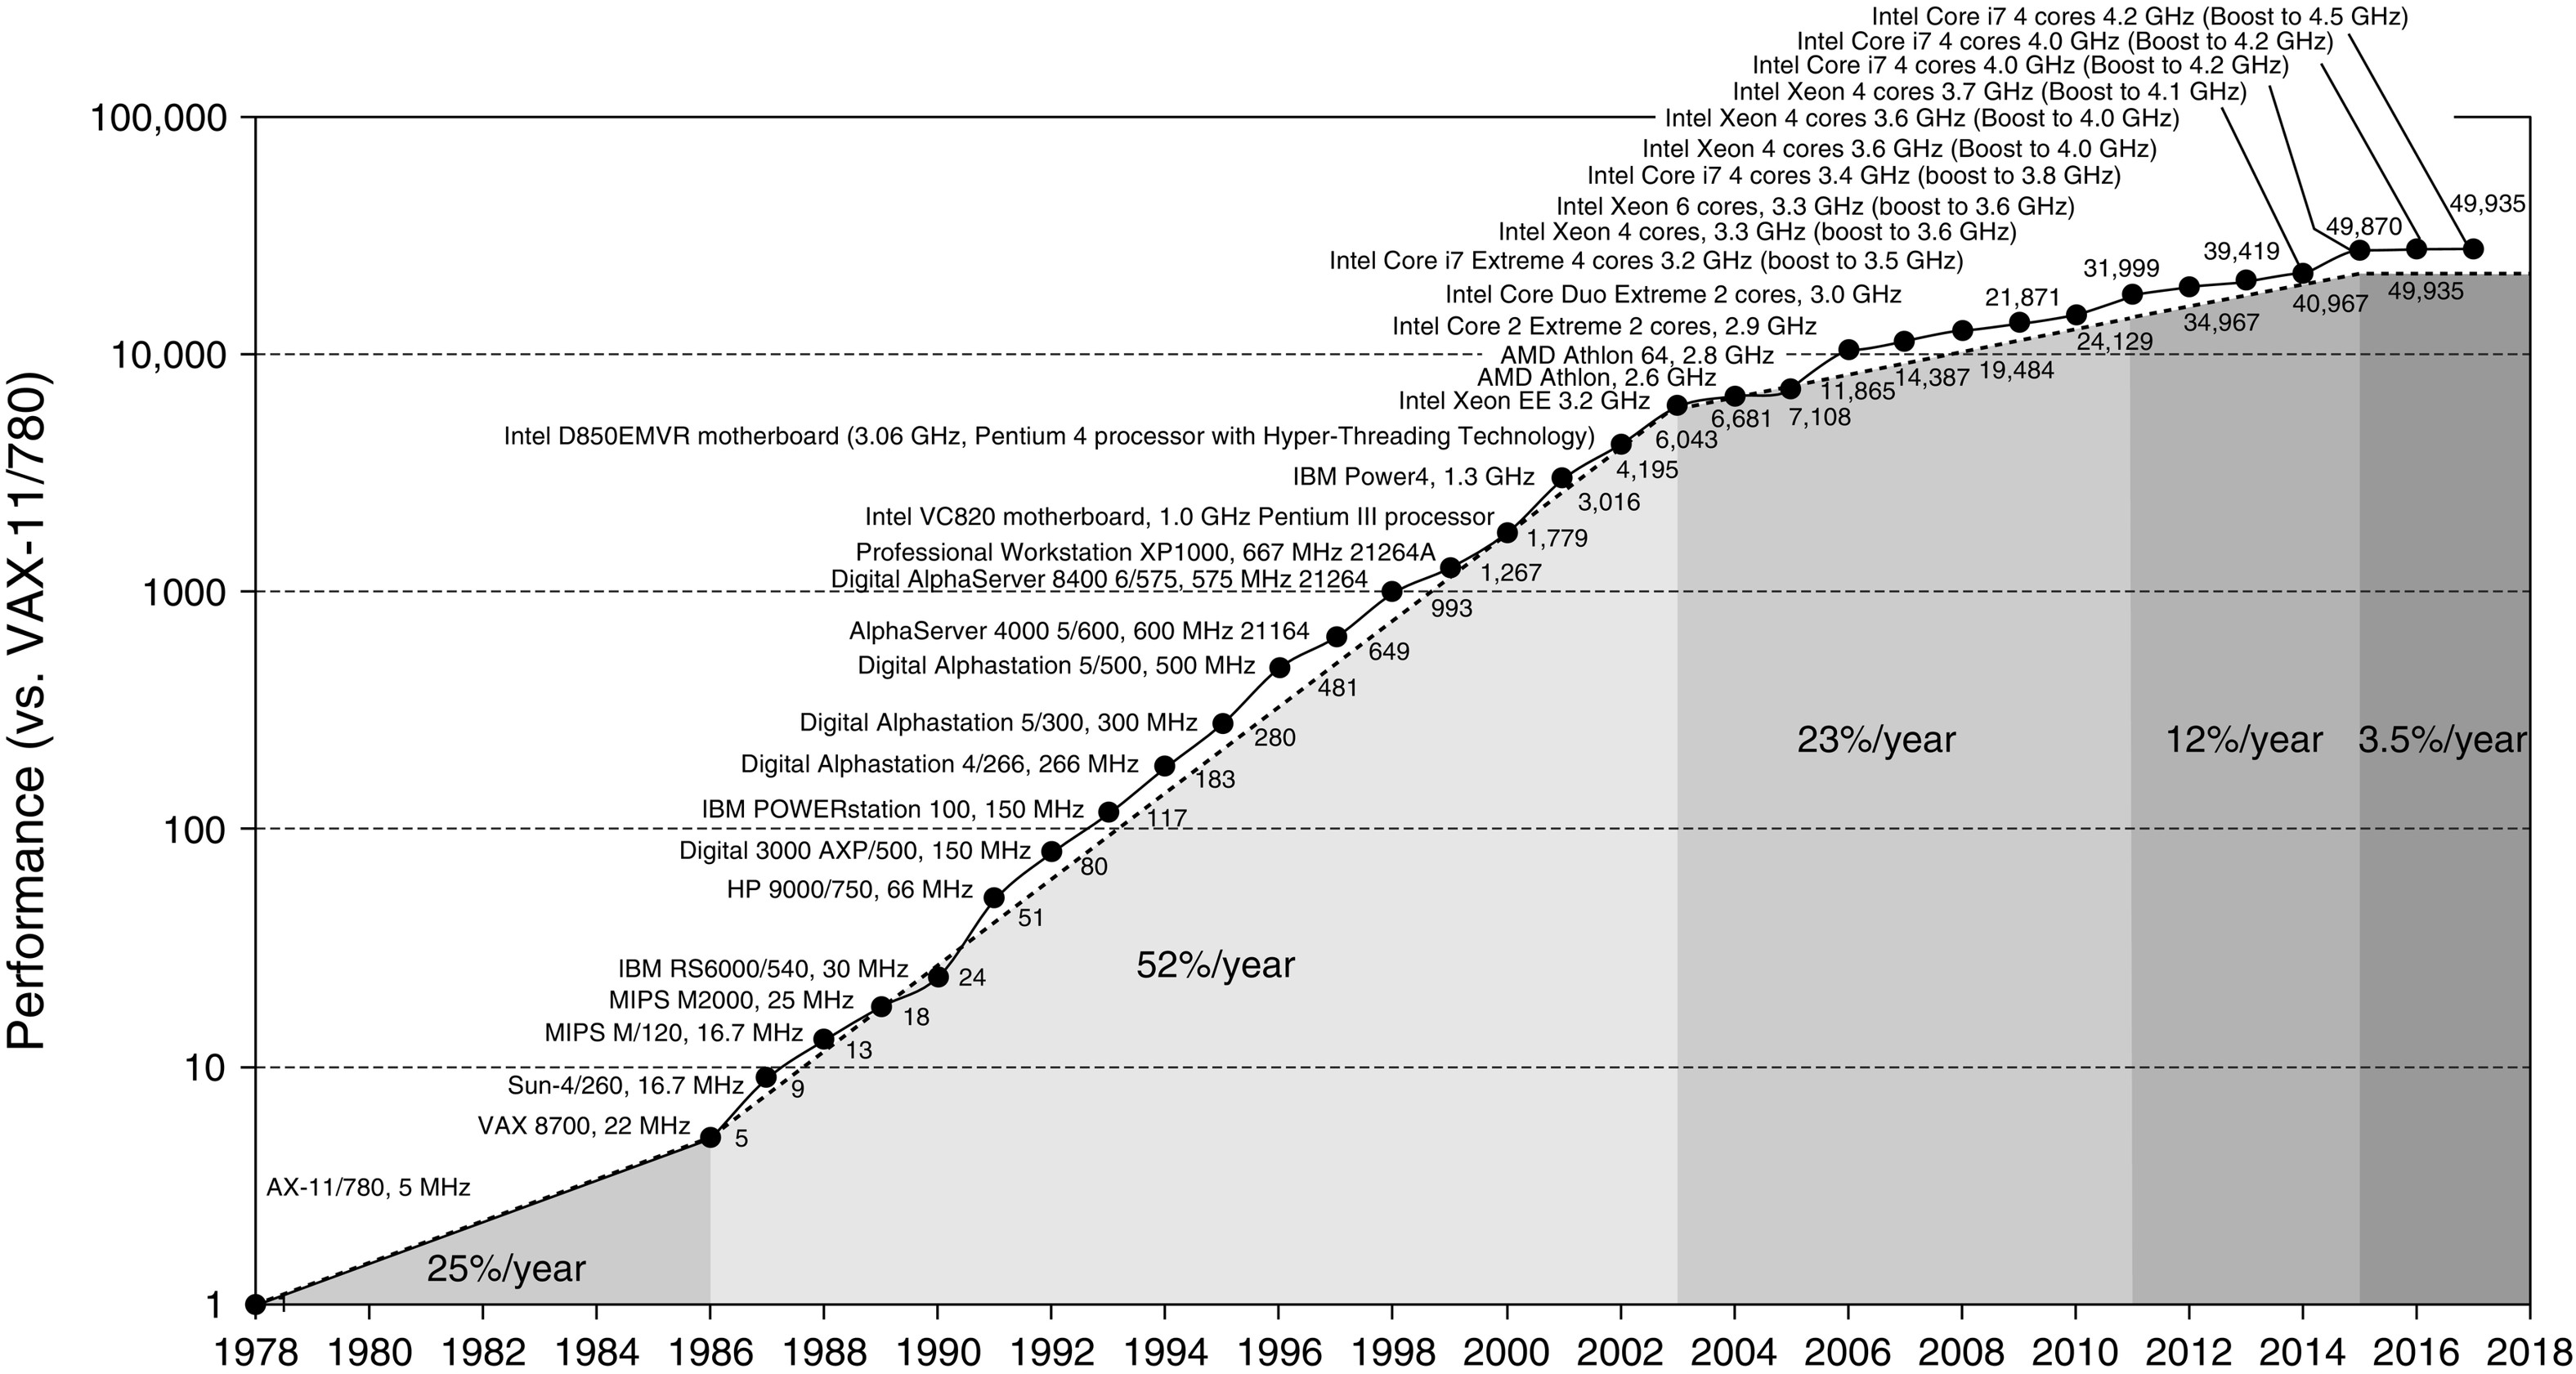
\includegraphics[width=0.8\textwidth]{../Immagini/Capitolo 1/PrestazioniProcessori}
    \caption{Crescita nelle prestazioni dei processori dal 1978 al 2018; il grafico riporta le prestazioni dei processori, paragonandoli al VAX11/780, mediante l'esecuzione dei \textit{benchmark} SPECint \small{\textit{(Da J.L. Hennessy, D.A. Patterson, Computer Architecture: A quantitative Approach. Ed. 6. Waltham, MA:Elsevier, 2017)}}}
    \label{fig:PrestazioniProcessori}
\end{figure}\newline
In futuro, il miglioramento delle prestazioni dei microprocessori sar\`a verosimilmente determinato dall'aumento del numero di \textit{core} montati su un singolo \textit{chip} piuttosto che dalla crescita della frequenza di \textit{clock} dei singoli processori.